\section{Design}

\subsection{Struttura}
Le due principali architetture di tipo client-server più utilizzate sono:
\begin{itemize}
    \item Architettura ad anello: non esiste un elemento centrale, i client si conoscono tra loro e formano un gruppo con topologia ad anello. I client conoscono quindi gli indirizzi di tutti gli altri, mantenendoli in modo persistente.
    Questo tipo di architettura risulta però fragile considerando i meccanismi di sicurezza di Internet. Inoltre, sono richiesti meccanismi avanzati per la gestione della comunicazione tra i nodi. Infine se il numero di client è elevato sono possibili ritardi.
    \item Architettura con server centrale: si tratta della tipica modalità client-server. Un server offre un servizio e i client effettuano richieste o si connettono ad esso.
    Il singolo client non vede e non conosce gli altri.
    Il server rappresenta il punto critico di tutta l'architettura. In caso di problemi o guasti non è possibile offrire il servizio a nessun client. D'altra parte la gestione dei messaggi di comunicazione risulta molto più semplice da gestire e da progettare.
\end{itemize}

\noindent L’architettura scelta per la realizzazione di questo progetto è stata la seconda.

\begin{figure}[H]
    \caption{Architettura ad alto livello}
    \centering
    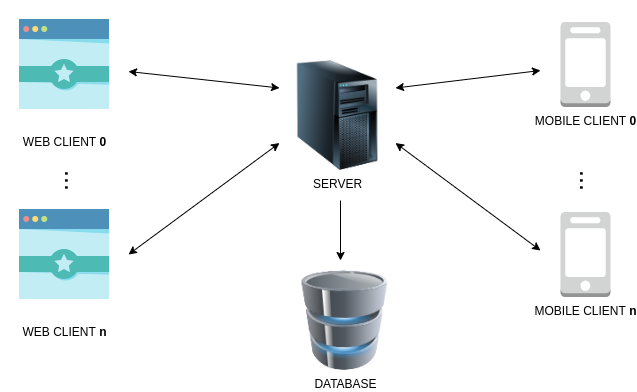
\includegraphics[width=120mm]{img/ingSoft/Architecture.png}
    \label{fig:base_architecture}
\end{figure}

\noindent Il server gestisce le richieste dei client e se necessario aggiunge/aggiorna/recupera dati dal Database.

\subsubsection{Struttura del Server}
In un'architettura con server centrale sono possibili due approcci differenti:
\begin{itemize}
    \item {\textbf{Stateless server}}\\
    Un server senza memoria di stato tratta ogni richiesta come una transazione indipendente rispetto ogni richiesta precedente.\newline
    Il vantaggio più grande offerto da questo approccio è la relativa semplicità nella progettazione del server; esso difatti non ha bisogno né di tenere in relazione transazioni diverse, né di allocare/deallocare dinamicamente un'area di memoria dedicata dedicata ai vari client.\newline
    D'altro canto la scelta di questo approccio porta intrinsecamente alcuni vantaggi come ad esempio la necessità di inviare un numero maggiore di dati in ogni richiesta.
    \item {\textbf{Stateful server}}\\
    Un server con memoria di stato, viceversa, risponde alle richieste dei client in modo coerente dipendentemente dallo stato attuale in cui si trova.\newline
    Al costo di un numero minore di dati scambiati tra client e server, si ottiene una gestione più complessa di problematiche quali la disconnessione di un client.
\end{itemize}
All'interno della nostra architettura si è scelto di optare per una versione stateful del server.
\paragraph{Diagramma delle classi}\mbox{}\\
Analizziamo ora il diagramma delle classi del server attraverso il quale potremo ottenere una comprensione di come esso mantenga la memoria di stato delle comunicazioni con i vari client.
\begin{figure}[H]
    \caption{Diagramma delle classi (Server)}
    \centering
    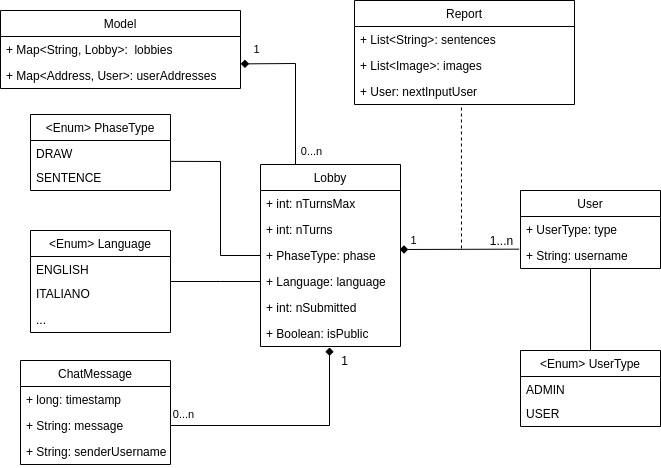
\includegraphics[width=150mm]{img/ingSoft/Class Server.png}
    \label{fig:class_server}
\end{figure}
\noindent La classe \emph{Lobby} è il cuore dello stato del server. Esisteranno molteplici istanze di Lobby, una per ogni lobby creata dagli utenti (i riferimenti ad essi saranno salvati nella classe contenitore \emph{Model}).\newline

\noindent In ogni Lobby sono presenti N \emph{User} (almeno uno, se la lobby rimane vuota il server procederà a rimuoverne l'istanza); ogni User è caratterizzato, oltre che dal suo username, dallo UserType. Ogni Lobby contiene un solo User di tipo ADMIN il quale inizialmente sarà necessariamente lo User creatore della Lobby (ma potrebbe cambiare in futuro se lo User di tipo ADMIN si disconnette).\newline

\noindent Ogni User, oltre ad avere un riferimento alla Lobby di appartenenza, sarà mappato per associarlo all'indirizzo attraverso il quale raggiungerlo tramite socket. Tale mapping avverrà nella classe contenitore Model.\newline

\noindent Lobby contiene inoltre tutti i dati per gestire la partita in corso (modificando il suo stato tramite il campo PhaseType); per ogni nuova partita collegata all'istanza di lobby verrà generato un \emph{Report} per ogni User. Tale Report conterrà al suo interno le frasi ed i disegni inviati dai giocatori (oltre che un riferimento al prossimo giocatore che dovrà "scrivere" su tale Report).\newline

\noindent Infine la Lobby contiene il riferimento ad N \emph{ChatMessage}; ogni istanza di tale classe memorizzerà l'istante temporale di invio del messaggio, il suo contenuto e l'username del mittente (non salverà il riferimento all'istanza dello User in quanto esso potrebbe uscire dalla Lobby ma i messaggi vanno preservati fino alla chiusura di quest'ultima).

\paragraph{Diagramma degli stati}\mbox{}\\
Vediamo ora il diagramma degli stati del server, così da comprendere come il suo stato vari nel tempo in base alle interazioni con i client.

\begin{figure}[H]
    \caption{Diagramma degli stati, parte 1(Server)}
    \centering
    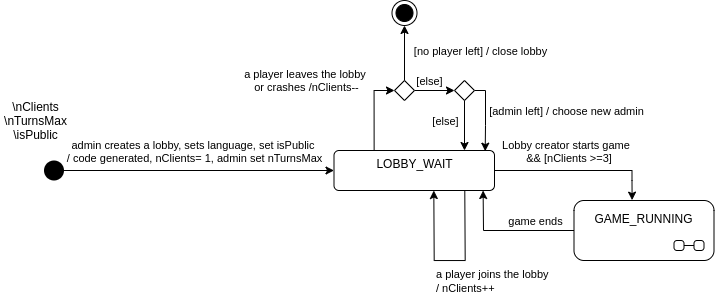
\includegraphics[width=150mm]{img/ingSoft/State Server.png}
    \label{fig:server_state}
\end{figure}

\noindent In questo diagramma troviamo due stati:
    \begin{itemize}
        \item {\textbf{Lobby wait}}\\
        Esso rappresenta lo stato in cui si trova la lobby quando è stata appena creata o quando la partita è terminata.
        \item {\textbf{Game running}}\\
        Uno stato composto rappresentante lo svolgimento della partita. Per comodità la composizione di tale stato verrà analizzata a breve.
    \end{itemize}
Un utente crea una lobby (divenendo admin) fornendo le sue impostazioni quali la lingua e se rendere la lobby pubblica o meno.\newline

\noindent Indipendentemente dalla visibilità di tale Lobby verrà generato un codice alfanumerico a sei caratteri univoco attraverso il quale gli utenti potranno connettersi alla lobby (nel caso la lobby abbia visibilità pubblica gli utenti potranno entrare anche cercando una lobby per lingua).\newline

\noindent Nel momento in cui un utente abbandoni la lobby (sia per sua volontà che per problemi di connessione), andranno effettuati dei controlli: innanzitutto verrà controllato il numero di giocatori rimasti; se non sarà rimasto nessun giocatore la lobby corrente verrà chiusa.\newline
Nel caso in cui sia rimasto almeno un utente, verrà controllato il tipo di utente disconnesso; se tale utente era l'admin della lobby, allora verrà eletto casualmente un admin tra gli utenti rimasti.\newline

\noindent La presenza di un admin risulta fondamentale in quanto egli (previa il soddisfacimento della condizione di almeno tre utenti connessi alla lobby) darà il via al gioco, facendo cambiare lo stato in Game running. Intuitivamente da tale stato si uscirà alla fine della partita, qualsiasi sia la causa della fine di essa.\newline

\noindent Vediamo ora nel dettaglio lo stato Game Running.

\begin{figure}[H]
    \caption{Diagramma degli stati, parte 2(Server)}
    \centering
    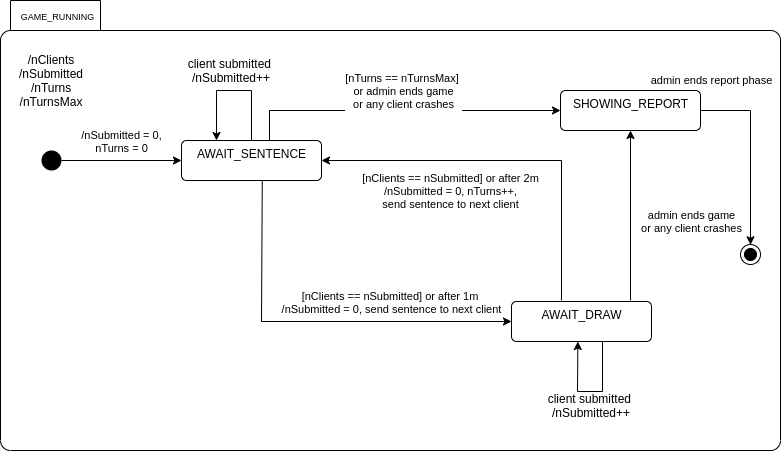
\includegraphics[width=150mm]{img/ingSoft/State Server Macro.png}
    \label{fig:server_state_2}
\end{figure}

\noindent Il macro-stato si compone di 3 stati interni:
\begin{itemize}
    \item {\textbf{Await sentence}}\\
    In questo stato il server attende che tutti gli utenti inviino le loro frasi, indipendentemente dal fatto che sia la prima frase o una che segua un disegno.
    \item {\textbf{Await draw}}\\
    Qui il server attende che tutti gli utenti inviino i loro disegni. Questo stato è necessariamente successivo alla Await sentence in quanto i disegni si riferiscono alla frase ricevuta.
    \item {\textbf{Showing report}}\\
    Al termine della partita vengono mostrati i report contenenti frasi e disegni di tutti i giocatori.
\end{itemize}
Prima di analizzarne il funzionamento è necessario chiarire il concetto di turno tramite un esempio pratico.\newline

\noindent Supponiamo di avere tre utenti: Alessandro, Piero e Angelo; inizialmente tutti gli utenti scrivono una frase a loro scelta. La frase dunque verrà inviata al successivo utente seguendo uno shift di uno verso destra (la frase di Alessandro verrà inviata a Piero, quella di Piero ad Angelo e quella di quest'ultimo ad Alessandro).\newline

\noindent I tre utenti dunque faranno un disegno rappresentante la frase ricevuta. Analogamente a prima, il disegno realizzato da Alessandro verrà inviato a Piero, quello di Piero ad Angelo e quello di Angelo ad Alessandro, così che gli utenti possano scrivere una frase dipendentemente dal disegno ricevuto.\newline

\noindent \emph{La scrittura di una frase e la realizzazione di un disegno  comporta il passaggio di un turno.} Questo significa che in una partita da quattro turni che si completi correttamente ogni utente avrà scritto quattro frasi e realizzato quattro disegni.\newline

\noindent Chiarito questo, durante la creazione verrà settato il numero di turni che andranno svolti nella partita (corrispondente alla variabile nTurnsMax nel diagramma).\newline
Entrando per la prima volta nello stato Await sentence, verranno inizializzate a zero due variabili:
\begin{itemize}
    \item \emph{nTurns}, rappresentante il numero di turni trascorsi
    \item \emph{nSubmitted}, rappresentante il numero di giocatori che hanno inviato la loro frase o, nel caso ci si trovi in Await draw, il loro disegno
\end{itemize}

\noindent Durante la Await sentence, ogni utente che invierà la sua frase aumenterà il valore di nSubmitted. Avverrà dunque una transizione ad Await draw quando tutti i client avranno inviato la loro frase o sarà trascorso un minuto (prendendo come frase il contenuto attuale della casella di testo). La transizione riporterà a zero il contatore nSubmitted e provvederà ad inviare le frasi ai destinatari corretti.\newline

\noindent In modo totalmente analogo, nello stato Await draw, ogni utente invia il proprio disegno incrementando nSubmitted. La transizione verso Await sentence avverrà quando tutti gli utenti avranno effettuato l'invio o saranno trascorsi due minuti. Anche qui il disegno sarà inoltrato al destinatario corretto e sarà portato a zero nSubmitted. In questo caso però sarà anche incrementato il contatore nTurns.\newline

\noindent Vi sono tre modi per transizionare \emph{VERSO} lo stato Showing report:
\begin{itemize}
    \item Il numero di turni massimo è stato raggiunto; effettueremo quindi una transizione da Await sentence a Showing report
    \item L'admin decide di interrompere prematuramente la partita (opzione disponibile solo durante lo stato Await sentence); effettueremo quindi una transizione da Await sentence a Showing report
    \item La connessione con un client qualsiasi viene interrotta; effettueremo quindi una transizione verso Showing report indipendentemente dal fatto che ci troviamo in Await sentence o Await draw
\end{itemize}

\noindent Dallo stato Showing report si uscirà per decisione dell'admin o nel caso non sia rimasto più nessun client.

\paragraph{Gestione della disconnessione dei client}\mbox{}\\
Come intuibile dalla spiegazione pregressa, la disconnessione di un client causa la terminazione della partita, se in corso, portando tutti i giocatori alla visione dei risultati.\newline
Questa scelta è stata presa data la natura del gioco che rende impossibile continuarlo quando un giocatore se ne va.\newline
Al fine di non perdere quanto fatto fino a quel momento, però, i giocatori vengono comuinque portati alla visione dei report per visionare quanto fatto fino al momento della disconnessione.

\subsubsection{Struttura del Client}
Alla luce di un'implementazione statefull del server, il lato client non mantiene lo stato, ma si limita ad adeguarsi alle istruzioni inviategli dal server.

\begin{figure}[H]
    \caption{Diagramma degli stati, parte 1 (Client)}
    \centering
    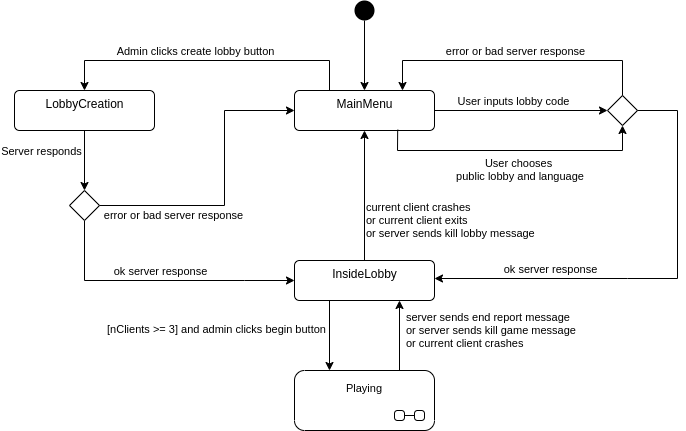
\includegraphics[width=150mm]{img/ingSoft/State Client.png}
    \label{fig:client_state_simple}
\end{figure}

\noindent Troviamo quattro stati:
\begin{itemize}
    \item {\textbf{Main menu}}\\
    L'utente si trova nel menu principale, da qui può decidere di creare una lobby o di partecipare ad una lobby già esistente.
    \item {\textbf{Lobby creation}}\\
    L'utente si trova nella fase di creazione della lobby e, in caso di successo, verrà inserito come Admin nella lobby appena creata.
    \item {\textbf{Inside lobby}}\\
    L'utente si trova all'interno della lobby (insieme ad altri giocatori, se presenti).\newline
    È possibile arrivare in questo stato, oltre che a seguito della creazione di una lobby, entrando in una lobby; tale processo può avvenire identificando la lobby tramite il codice univoco o cercando una lobby pubblica casuale filtrando sulla lingua impostata.
    \item {\textbf{Playing}}\\
    Una volta che all'interno della lobby saranno disponibili almeno tre giocatori, il server sbloccherà la possibilità di cominciare il gioco; tale azione sarà resa disponibile solamente all'Admin. Anche in questo caso, per semplicità, lo stato Playing è in realtà uno stato composto.
\end{itemize}

\begin{figure}[H]
    \caption{Diagramma degli stati, parte 2 (Client)}
    \centering
    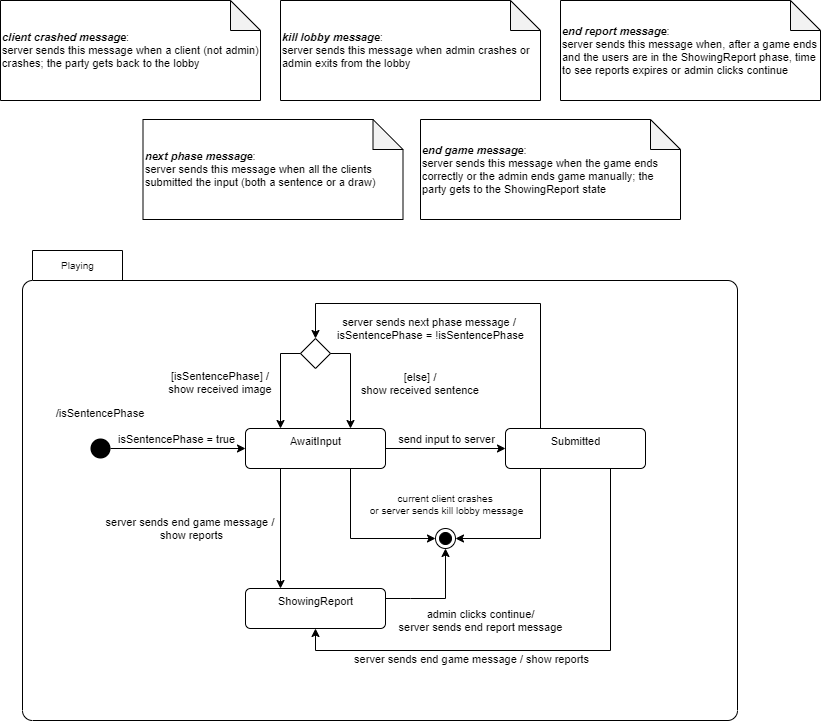
\includegraphics[width=150mm]{img/ingSoft/State Client Macro.png}
    \label{fig:client_state}
\end{figure}

\noindent In questo diagramma, che rappresenta la composizione dello stato Playing, sono presenti tre stati:
\begin{itemize}
    \item {\textbf{Await input}}\\
    In attesa dell'input dell'utente (frase o disegno).
    \item {\textbf{Submitted}}\\
    L'utente ha inviato il suo input (frase o disegno).
    \item {\textbf{Showing report}}\\
    La partita è terminata, è possibile visionare i report di tutti i giocatori.
\end{itemize}
Inizialmente viene settata una variabile booleana \emph{isSentencePhase} che indica se l'attuale input sia la frase (nel caso sia falsa significa che la fase attuale è la fase di disegno).\newline

\noindent Una volta che l'utente ha inviato il suo input, avviene la transizione verso lo stato Submitted nel quale l'utente rimarrà finchè non riceverà un messaggio dal server notificando che tutti gli utenti hanno inviato il loro input. La variabile isSentencePhase verrà negata, cambiando fase.\newline

\noindent Verrà eseguita una transizione verso Showing report nel caso il server invii un messaggio di fine partita; da qui, una volta che l'admin avrà cliccato sull'apposito bottone, il server notificherà a tutti i client connessi alla lobby l'uscita dallo stato Showing report, terminando il macro stato Playing.\newline

\noindent Nel caso il client perda la connessione, si ritroverà nel menu principale; i client ancora connessi invece riceveranno un messaggio dal server che imporrà di transizionare immediatamente allo stato Showing report.\newline

\subsubsection{Struttura del Database}
Il database deve essere in grado di memorizzare gli utenti che si registrano al sistema e mantenere in memoria i dati delle partite passate.\newline
L'entità \textit{User} mantiene i dati degli utenti, in particolare contiene i campi username e password. Sono stati omessi campi ulteriori come la e-mail per semplicità.\newline L'entità \textit{Game} mantiene solo i timestamp di inizio e fine partita.\newline
Le istanze della relazione rappresentanti gli utenti nella partita contengono anche il percorso del report finale.\newline
I disegni e le frasi scritte dagli utenti infatti vengono inserite in un file generato e mantenuto dal server.\newline
Inizialmente si era pensato di creare altre due entità per mantenere le immagini e le frasi, in modo da far generare il report al server solo al momento dello scaricamento, per poi cancellarlo.\newline
Questa idea è stata scartata per i seguenti motivi:
\begin{itemize}
    \item Le informazioni contentute nelle due tabelle sarebbero risulatte molto scarsamente riutilizzabili a causa della natura dell'applicazione;
    \item Le informazioni all'interno delle tabelle sono inutili se trattate da sole;
\end{itemize}
\begin{figure}[H]
    \caption{Struttura del Database (ER - Logico)}
    \centering
    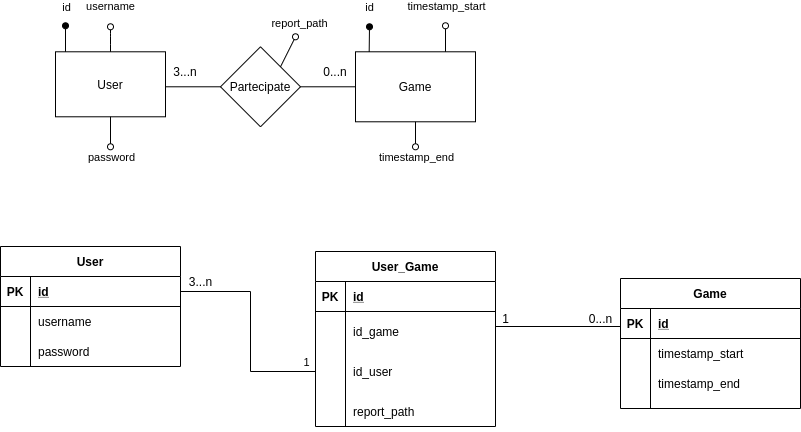
\includegraphics[width=150mm]{img/ingSoft/ER - Logic.png}
    \label{fig:db_struct}
\end{figure}

\subsubsection{WireFrame}
In questa sezione verranno illustrati i Wireframe dell'applicazione, realizzati durante la fase di progettazione.
Tutte le schermate dell'applicazione sono state progettate con un'ottica mobile-first, ovvero puntando all'ottimizzazione del design su dispositivi mobili.\newline
In tutte le schermate compare una NavBar in cui compare il Logo dell'applicazione, una Label che indica il nome della pagina in cui ci si trova e un'icona rappresentante operazioni possibili per l'utente (per esempio il Logout).\newline
La prima pagina che compare quando si accde all'applicazione è la schermata di Autenticazione (Wireframe mancante). In questa schermata è possibile effettuare la registrazione di un nuovo account o il login. Qualora si effettuasse una registrazione verrà effettuato in automatico anche il Login. Inserendo le proprie credenziali in modo corretto e cliccando sul pulsante Login si potrà accedere al menù principale.\newline
In caso di credenziali sbagliate l'utente viene avvertito e viene invitato a provare di nuovo.

Nella schermata del menù Principale l'utente può cliccare su quattro pulsanti.
\begin{itemize}
    \item \textbf{Create Lobby}: Reindirizza l'utente alla pagina di creazione di una Lobby;
    \item \textbf{Join Random Lobby}: Fa comparire una schermata in cui l'utente deve inserire la propria lingua per poter entrare una Lobby casuale in cui gli utenti parleranno la sua stessa lingua;
    \item \textbf{Join Specific Game}: Fa comparire una schermata in cui l'utente deve inserire il codice identificativo di una lobby già creata;
    \item \textbf{Show previous Report}: Reindirizza l'utente alla pagina in cui può scaricare e consultare i report delle partite che ha giocato in passato.
\end{itemize}

\begin{figure}[H]
    \caption{Wireframe del Menu Principale.}
    \centering
    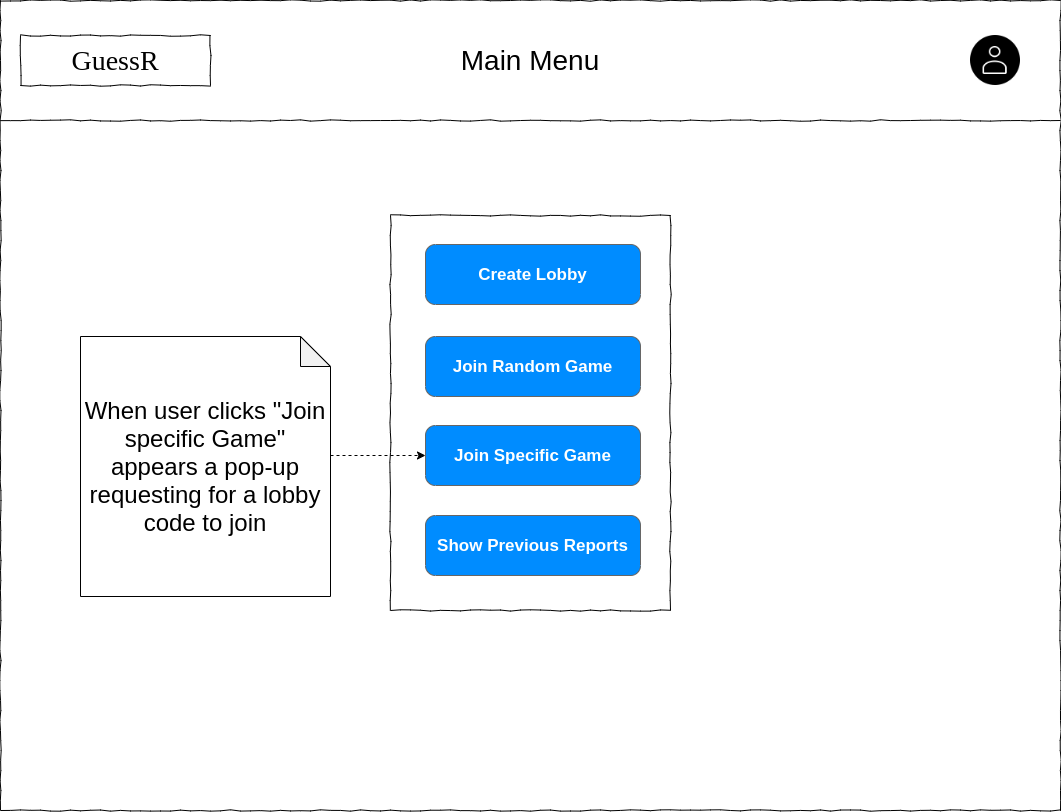
\includegraphics[width=150mm]{img/ingSoft/wireframeMainMenu.png}
    \label{fig:main_menu_wireframe}
\end{figure}

\noindent Premendo sul pulsante \textit{Create Lobby} compare la pagina di creazione di una Lobby. Questa pagina contiene un Form in cui è possibile impostare i parametri della Lobby. L'interruttore ``Set Visibilty" permette di impostare la visibilità della Lobby. Se si imposta la Lobby come privata solo gli utenti che posseggono il codice di accesso possono accedere. Se si imposta la lobby come pubblica qualsiasi utente potrà entrare nella Lobby.
È poi possibile inserire il numero di turni che si desidera giocare (un turno è definito come l'input sequenziale di una frase e un disegno da parte di tutti gli utenti). Infine è necessario selezionare la lingua in cui si vuole giocare tra le possibili offerte. Il pulsante \textit{"Create Lobby"} reindirizza l'utente alla pagina in cui attende che altri utenti accedano alla lobby per poter giocare.
\begin{figure}[H]
    \caption{Wireframe (Creazione della lobby)}
    \centering
    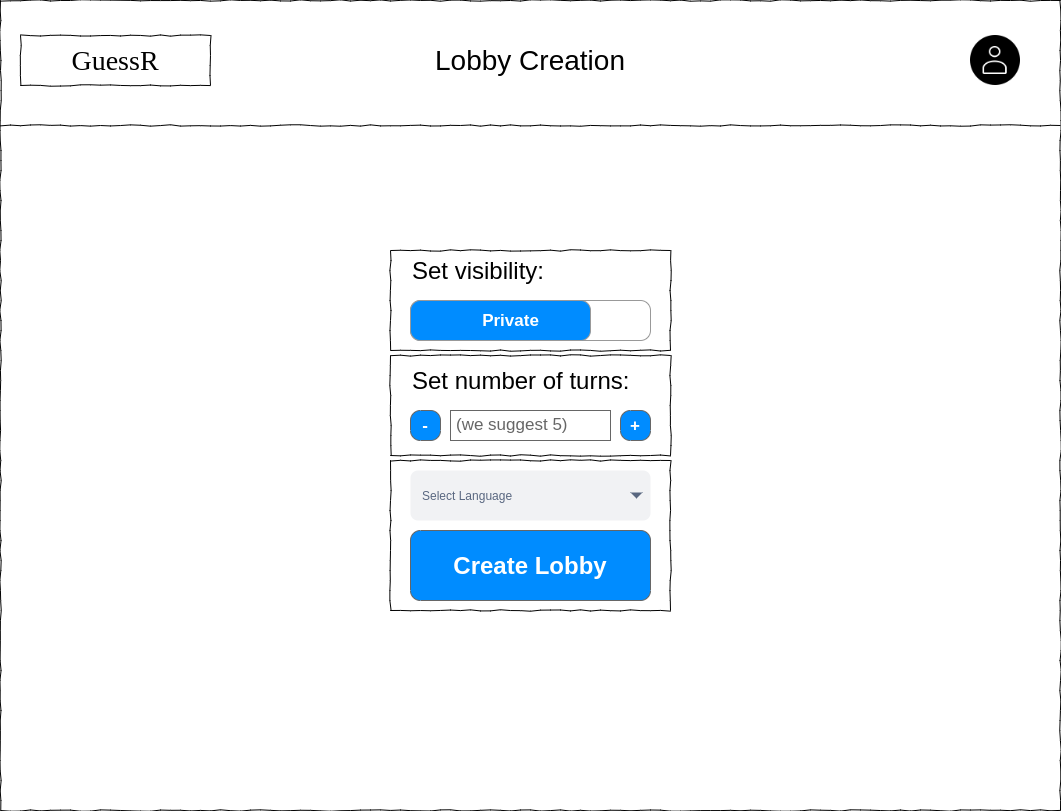
\includegraphics[width=150mm]{img/ingSoft/wireframeCreation.png}
    \label{fig:lobby_create_wireframe}
\end{figure}

\noindent Nella schermata della Lobby creata compare il codice univoco assegnato alla Lobby sulla NavBar. Nella parte centrale dello schermo vengono illustrate le regole del gioco. Nella parte sinistra dello schermo compaiono i messaggi inviati dagli utenti ed il form utilizzato per mandarli. Nella parte destra dello schermo compare la lista dei giocatori all'interno della Lobby.
Infine, sotto le regole del gioco è presente un pulsante ``Exit Lobby" che se premuto fa uscire l'utente dalla Lobby. Un pulsante aggiuntivo ``Start Game" compare solo all'utente che ha creato la Lobby (l'utente di tipo Admin). Se premuto, questo pulsante reindirizza tutti gli utenti all'interno della Lobby alla schermata di Gioco.

\begin{figure}[H]
    \caption{Wireframe (Lobby creata)}
    \centering
    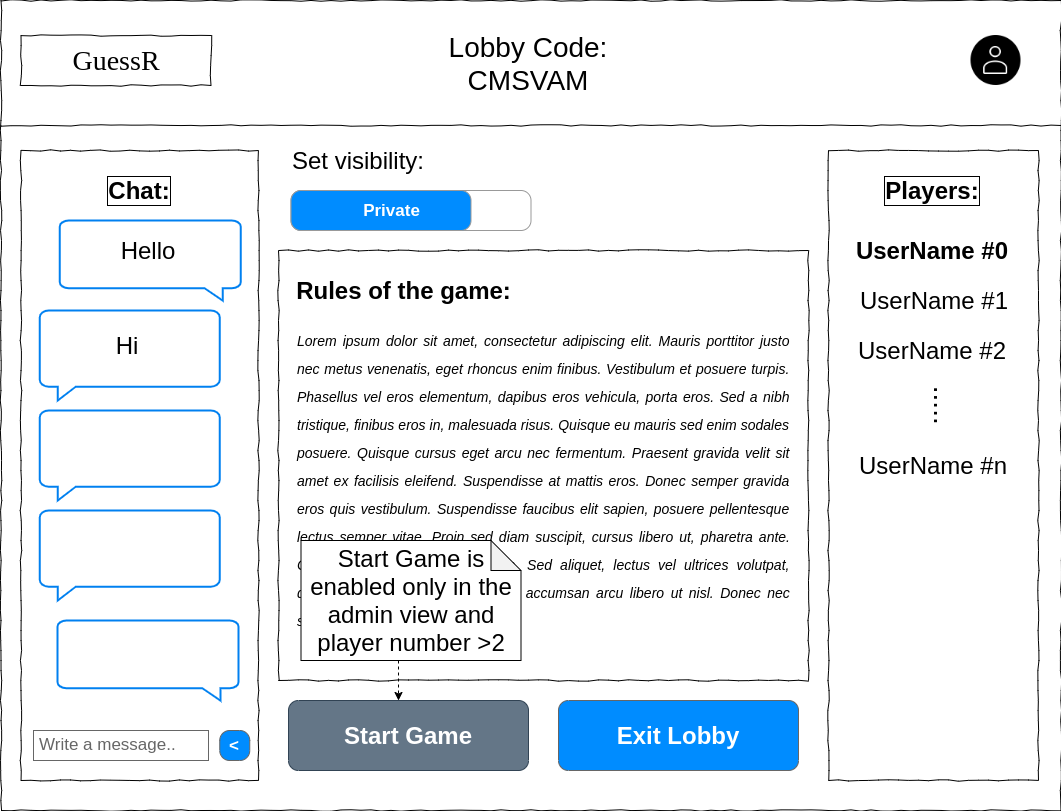
\includegraphics[width=150mm]{img/ingSoft/wireframeInLobby.png}
    \label{fig:inside_lobby_wireframe}
\end{figure}

\noindent Nella schermata di gioco la parte destra e sinistra dello schermo rimane immutata rispetto alla pagine precedente. È quindi ancora possibile consultare ed inviare messaggi sulla chat e vedere i giocatori che stanno giocando.\newline
Sulla NavBar viene illustrata la fase di gioco.
\begin{itemize}
    \item Se la fase è \textit{``Sentence"} l'utente dovrà digitare una frase a suo piacimento (al primo turno o nel caso in cui non abbia ricevuto alcun disegno) o una frase che rappresenta in disegno che vede a schermo nel box di testo.
    \item Se la fase è \textit{``Draw"} l'utente dovrà disegnare come meglio possibile ciò che legge nella frase ricevuta.
    Il disegno va eseguito nell'apposito box bianco messo a disposizione.
\end{itemize}

\begin{figure}[H]
    \caption{Wireframe (Giocando)}
    \centering
    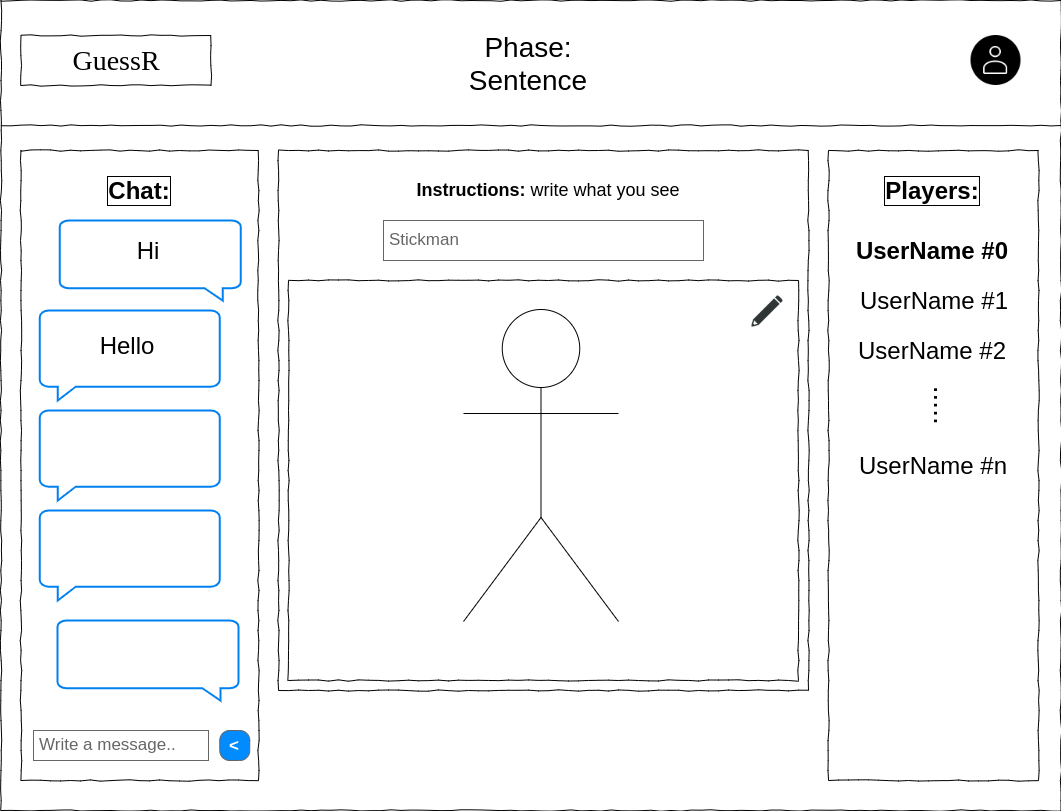
\includegraphics[width=150mm]{img/ingSoft/wireframeInGame.png}
    \label{fig:playing_wireframe}
\end{figure}

\noindent Quando il numero di turni finisce o un utente si disconnette tutti gli utenti vengono reindirizzati alla pagina in cui vengono visualizzati tutti i fogli (o report). Anche in questa pagina è presente un pulsante ``Exit Lobby" per uscire dalla Lobby. L'utente che ha creato la lobby ha a disposizione un ulteriore pulsante ``Back to Lobby" che reindirizza tutti gli utenti alla pagine in cui si attende che altri giocatori entrino nella Lobby.

\begin{figure}[H]
    \caption{Wireframe Mobile (Giocando)}
    \centering
    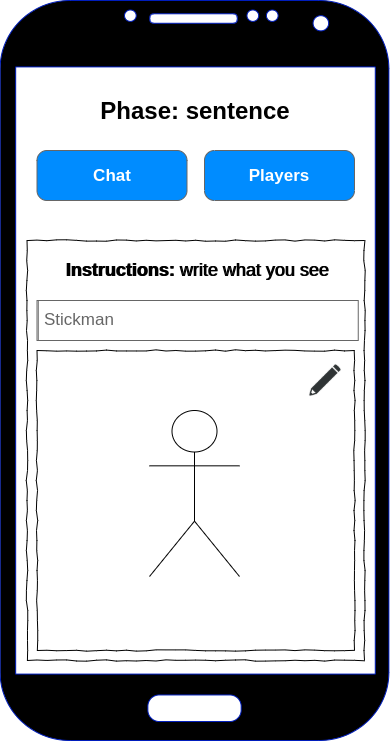
\includegraphics[width=50mm]{img/ingSoft/wireframeMobileInGame.png}
    \label{fig:playing_mobile_wireframe}
\end{figure}

\noindent La maggior parte delle pagine contengono poco contenuto, fatta eccezione per le pagine in cui compaiono la chat e la lista degli utenti.\newline
Proprio questi due elementi, nella versione mobile dell'applicativo vengono condensati in due bottoni. Cliccando sui bottoni ``Chat" e ``Players" si apriranno dei pop-up che mostreranno le informazioni in un formato più consono alla dimensione dello schermo.

\subsection{Comportamento}
%
\subsubsection{DatabaseVerticle [Abstract]}
Si tratta di una classe astratta che a sua volta estende AbstractVerticle. Ogni Verticle che necessita di una connessione al Database estenderà quest'ultima al posto di AbstractVerticle in modo che si possa connettere agevolmente con il Database MySql. La comodità risiede nel riuso di codice e nella facilità di modifiche per tutti gli aspetti concernenti il Database.

\subsubsection{ApiVerticle}
Si tratta del Verticle che si occupa di restituire dati di diversa natura (elenco delle lingue, lista dei report e singoli report) agli utenti che ne fanno richiesta. Tutte le routes che gestisce questo Verticle impiegano il metodo GET. Questa classe estende DatabaseVerticle per accedere al Database per le operazioni che hanno come oggetto i report ed effettuare query di ricerca su tali.

\subsubsection{AuthVerticle}
E' il Verticle che gestisce il servizio di autenticazione degli utenti nel sistema, gestendone la registrazione e l'accesso (Log in). Si troverà pertanto a dialogare con il Database (estende DatabaseVerticle) e a dover effettuare query per l'inserimento di utenti e per la ricerca di tali qualora siano già registrati.

\subsubsection{GameDataStoreVerticle}
GameDataStoreVerticle si occupa di immagazzinare informazioni riguardanti le partite concluse, pertanto anch'esso estende DatabaseVerticle ed effettua delle query di inserimento nelle tabelle di "game" e di "user\_game". Al termine di ogni partita la richiesta per effettuare l'upload dei dati di gioco deve essere effettuata dall'utente con ruolo di amministratore della lobby, e non può essere effettuata da utenti normali. Questa classe permette anche la generazione dei report a partire dai messaggi che arrivano al server al termine di una partita.

\subsubsection{MainVerticle}
Si tratta del Verticle principale, si occupa del deployment degli altri Verticle ed instrada le richieste sull'eventbus, in modo che gli altri Verticle le vedano e riescano a soddisfare le richieste in arrivo.

\subsection{Interazione}
%descrive the methods used to communicate
Le interazioni nell'applicativo partono da un client che si interfaccia al sistema in oggetto. Esso si ritroverà a registrarsi (sign up) o effettuare il login se già in possesso di un account. Una volta effettuato il login e convalidato dal servizio di autenticazione l' utente accede alla home ed ha la possibilità di creare una nuova lobby, determinando alcune sue caratteristiche tra cui la visibilità (lobby pubblica/privata), la lingua scelta con cui comunicare con gli altri utenti ed il numero di turni per cui il gioco continuerà prima di terminare (con un minimo di un turno), il server una volta ricevuta la richiesta di creazione da parte del client restituirà un messaggio di ok provvedendo un codice di 6 caratteri alfanumerici per la lobby. \newline

\noindent Una volta creata la lobby l'utente in questione prende il ruolo di Admin. Dalla schermata home ogni utente può anche prendere parte a lobby già esistenti, nel caso di pubbliche ricercando tramite "join random game" quelle esistenti per lingua, per lobby private immettendo il codice alfanumerico identificativo della lobby. \newline

\noindent Un utente che prende parte ad una lobby già esistente entrerà con il ruolo di User. Una volta che gli utenti desiderati hanno preso parte alla lobby, il suo Admin potrà provvedere a far partire il gioco comunicandolo al server.\newline

\begin{figure}[H]
    \caption{Diagramma di sequenza (Accesso alla Lobby)}
    \centering
    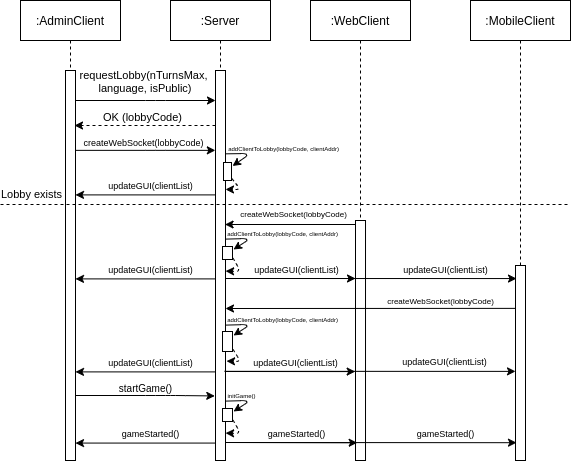
\includegraphics[width=150mm]{img/ingSoft/Sequence Lobby.png}
    \label{fig:sequence_lobby}
\end{figure}


\noindent Le restanti interazioni tra il client e il server riguardando l'alternarsi delle fasi di gioco, per cui ogni utente inizierà da una fase di "sentence" in cui sarà tenuto a inviare una frase che sarà poi oggetto di disegno per un altro giocatore, e così via per ogni giocatore. Una volta terminato il disegno un'ulteriore giocatore successivo dovrà ricostruire la frase iniziale a sua volta inviandone una appena prodotta. \newline

\noindent Ogni utente poi, una volta interagito con il sistema e aver giocato può scaricare i pdf autogenerati dei suoi report (composti da frasi e relativi disegni) che sono stati prodotti in partita, accedendo alla schermata "show reports" dalla home.

\begin{figure}[H]
    \caption{Diagramma di sequenza (Gioco)}
    \centering
    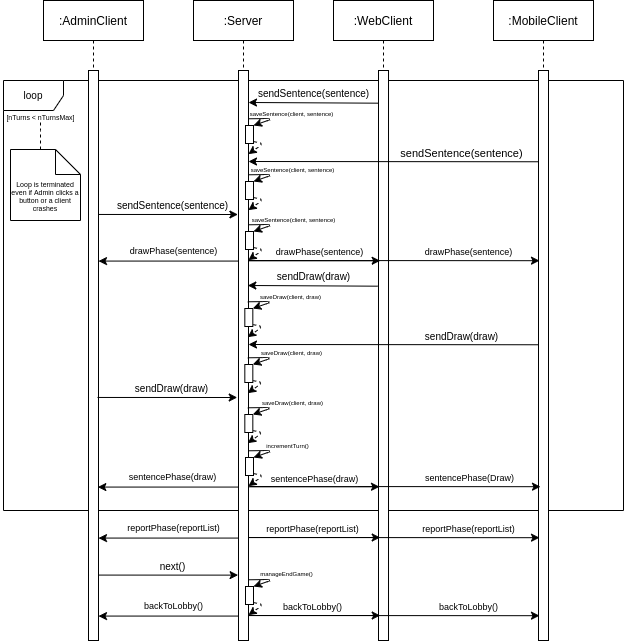
\includegraphics[width=150mm]{img/ingSoft/Sequence Game.png}
    \label{fig:sequence_game}
\end{figure}

\subsubsection{WebSocket Communication}
Grazie alle WebSocket è possibile instaurare connessioni full-duplex attraverso una singola connessione TCP.\newline
WebSocket è disegnato per essere implementato sia lato browser che lato server, ma può essere utilizzato anche da qualsiasi applicazione client-server.\newline
L'utilizzo delle WebSocket è particolarmente consigliato quando è necessaria una forte e ricorrente interazione tra client e server. Il loro utilizzo permette di semplificare notevolmente la realizzazione di applicazioni che forniscono contenuti e giochi in tempo reale.\newline
Nel caso di GuessR le Websocket vengono inizializzate sempre dal client che fa richiesta al server nel momento in cui un utente vuole creare una Lobby o accedere ad una già esistente.
L'utilizzo delle WebSocket è limitato ai momenti in cui un utente si trova all'interno di una lobby. La connessione termina nel momento in cui un utente esce dalla lobby o si disconnette per altri motivi (crash, cambio volontario o involontario di rete etc.).

\subsubsection{Socket Server Side}
Tutti gli eventi relativi alle connessioni con le web-socket avvengono sulla route ``/eventbus".\newline
È sempre il client ad inizializzare la connessione.\newline

\noindent Una socket può trovarsi in uno dei seguenti stati:
\begin{itemize}
    \item \textbf{SOCKET\_PING}: la socket è in uno stato simile definibile come idle in cui non sta succednendo nulla. Vengono inviati in polling messaggi di ping per verificare che la connessione sia ancora attiva;
    \item \textbf{SEND}: La websocket ha inviato un mesaggio (lato server il cambiamento di stato in SEND significa che una WebSocket ha inviato un messaggio, non che il server lo ha inviato);
    \item \textbf{RECEIVE}: La websocket ha ricevuto un messaggio(lato server il cambiamento di stato in RECEIVE significa che una WebSocket ha ricevuto un messaggio, non che il server lo ha ricevuto);
    \item \textbf{SOCKET\_CREATED}: La socket è appena stata creata;
    \item \textbf{REGISTERED}: La socket è appena stata registrata; Solitamente questa transizione di stato avviene dopo la creazione della socket;
    \item \textbf{UNREGISTER}: Viene annullata la registrazione della socket. Solitamente questa transizione di stato avviene prima della chiusura della socket;
    \item \textbf{SOCKET\_CLOSED}: La socket viene chiusa e termina il suo ciclo di vita.
\end{itemize}
\noindent Quando una socket cambia stato viene notificato nella route ed è possibile gestire tramite handler i comportamenti da eseguire ad ogni transizione.
\begin{info}[Info aggiuntive:]
Quando per esempio una socket viene creata ed entra nello stato \textbf{SOCKET\_CREATED} l'handler assegnato si occupa di aggiungerla alla collezione di socket attive.
Quando il client richiede la creazione di una WebSocket al server, quest'ultimo crea un oggetto di tipo SockJSSocket e la assegna all'utente corrispondente, scelto in base al contenuto del payload iniziale.\newline
Quando invece lo stato passa a \textbf{SOCKET\_CLOSED} la socket viene rimossa dalla collezione.
Quando al server arriva un messaggio (\textbf{SEND}, non \textbf{RECEIVE}) l'handler deve gestire il messaggio cercando di capire quale operazione eseguire in base al suo contenuto.
\end{info}
Utilizzando la classe \textit{SockJSBridgeOptions} è possibile specificare un filtro per il tipo di messaggi in entrata ed in uscita. In questo modo è possibile creare un insieme finito di tipi di messaggi ed assegnare a ciascuno un tipo di Handler.
I messaggi permessi sono stati contrassegnati nel seguente modo:
\begin{itemize}
    \item \textbf{USERNAME}: Gestisce le operazioni di creazioni e di accesso alle Lobby;
    \item \textbf{LOBBY}: Gestisce le operazioni che modificano lo stato della Lobby;
    \item \textbf{SENTENCE}: Gestisce i messaggi riguardanti l'invio di messaggi contenenti le frasi inviate dagli utenti;
    \item \textbf{DRAW}: Gestisce i messaggi riguardanti l'invio di messaggi contenenti i disegni inviati dagli utenti;
    \item \textbf{CHAT}: Gestisce i messaggi riguardanti la chat.
\end{itemize}

\noindent Utilizzando il metodo \textit{write()} sulla SockJSSocket è possibile per il server mandare messaggi ai relativi client. La natura del progetto richiede l'invio simultaneo di messaggi ad un'insieme specifico di client.\newline
Per questo motivo è stata sviluppata la classe d'utilità \textit{BroadcastUtility} che contiene il metodo statico \textit{sendMsgToSockets(sockets: Set<SockJSSocket>, msg: JsonObject)} che manda lo stesso messaggio ad un determinato insieme di Socket, generalmente, filtrate in base alla Lobby di appartenenza dell'utente.

\begin{figure}[H]
    \caption{Funzionamento di sendMsgToSockets()}
    \centering
    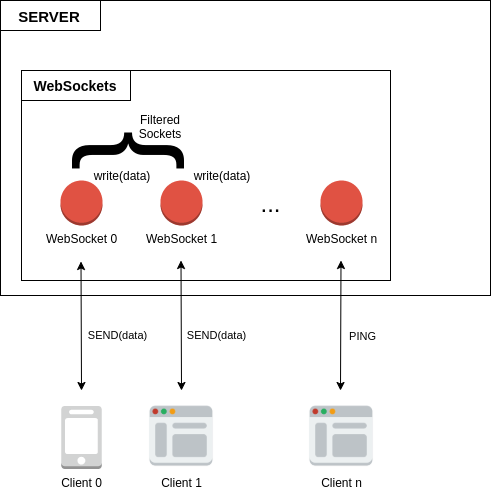
\includegraphics[width=120mm]{img/general/broadcast.png}
    \label{fig:send_message}
\end{figure}

\subsubsection{Socket Client Side}
Il collegamento tramite WebSocket da parte dei client avviene tramite i componenti denominati \textit{eventbusHandler}.\newline
Quando un componente eventBusHandler viene renderizzato (quando si crea una lobby o vi si accede) viene creato un oggetto EventBus che si collega alla path del server dedicata alle connessioni delle websocket.
\begin{minted}{js}
    var eventbus = new EventBus(serverUrl + '/eventbus');
\end{minted}
Creando questo oggetto viene anche inizializzata una websocket. È poi possibile come sul server gestire i tipi di messaggi in arrivo tramite handlers.
\begin{minted}{js}
    eventbus.registerHandler("messageType", function (error, message) {
        //...
    });
\end{minted}
È possibile inviare messaggi tramite il comando:
\begin{minted}{js}
    eventbus.send("messageType", body);
\end{minted}
Ed è possibile specificare le operazioni da effettuare quando la socket viene chiusa.
\begin{minted}{js}
    eventbus.onclose = function () {
        //...
    }
\end{minted}
I metodi di comunicazione sono quindi molto simili a quelli utilizzati all'interno del server. L'unica differenza risiede nella sintassi.

\subsection{Design scartato}
Inizialmente era stata presa in considerazione l'idea di realizzare il sistema in maniera differente da come appena illustrato.\newline
L'idea consisteva nel non inserire la logica di gioco all'interno del server ma all'interno di un solo client, che diventava una specie di mini-server per gli altri client che si connettevano a lui.\newline
Il server centrale sarebbe servito solo come intermediario per mettere in contatto i client tra loro e per gestire le varie richieste REST presenti nel progetto finale.\newline
Al fine di ottenere tale comportamento era stata presa in considerazione la tecnica del TCP hole punching, al fine di superare le limitazioni date dall'esistenza del NAT.\newline
Dopo aver notato la difficoltà nel mettere in contatto due client tra loro in modalità P2P l'idea è stata scartata.\newline
È inoltre importante menzionare il fatto che in un'architettura client-server i client dovrebbero contenere una quantità minima se non nulla di logica.
\newpage
